\section{Design}\label{design}

% System Architecture (Your idea)
% • Prototyping (how you implemented it)
% • Testing (how you are going to test it → Result)

\subsection{Architecture}\label{architecture}

\begin{figure}[h]
  \begin{center}
    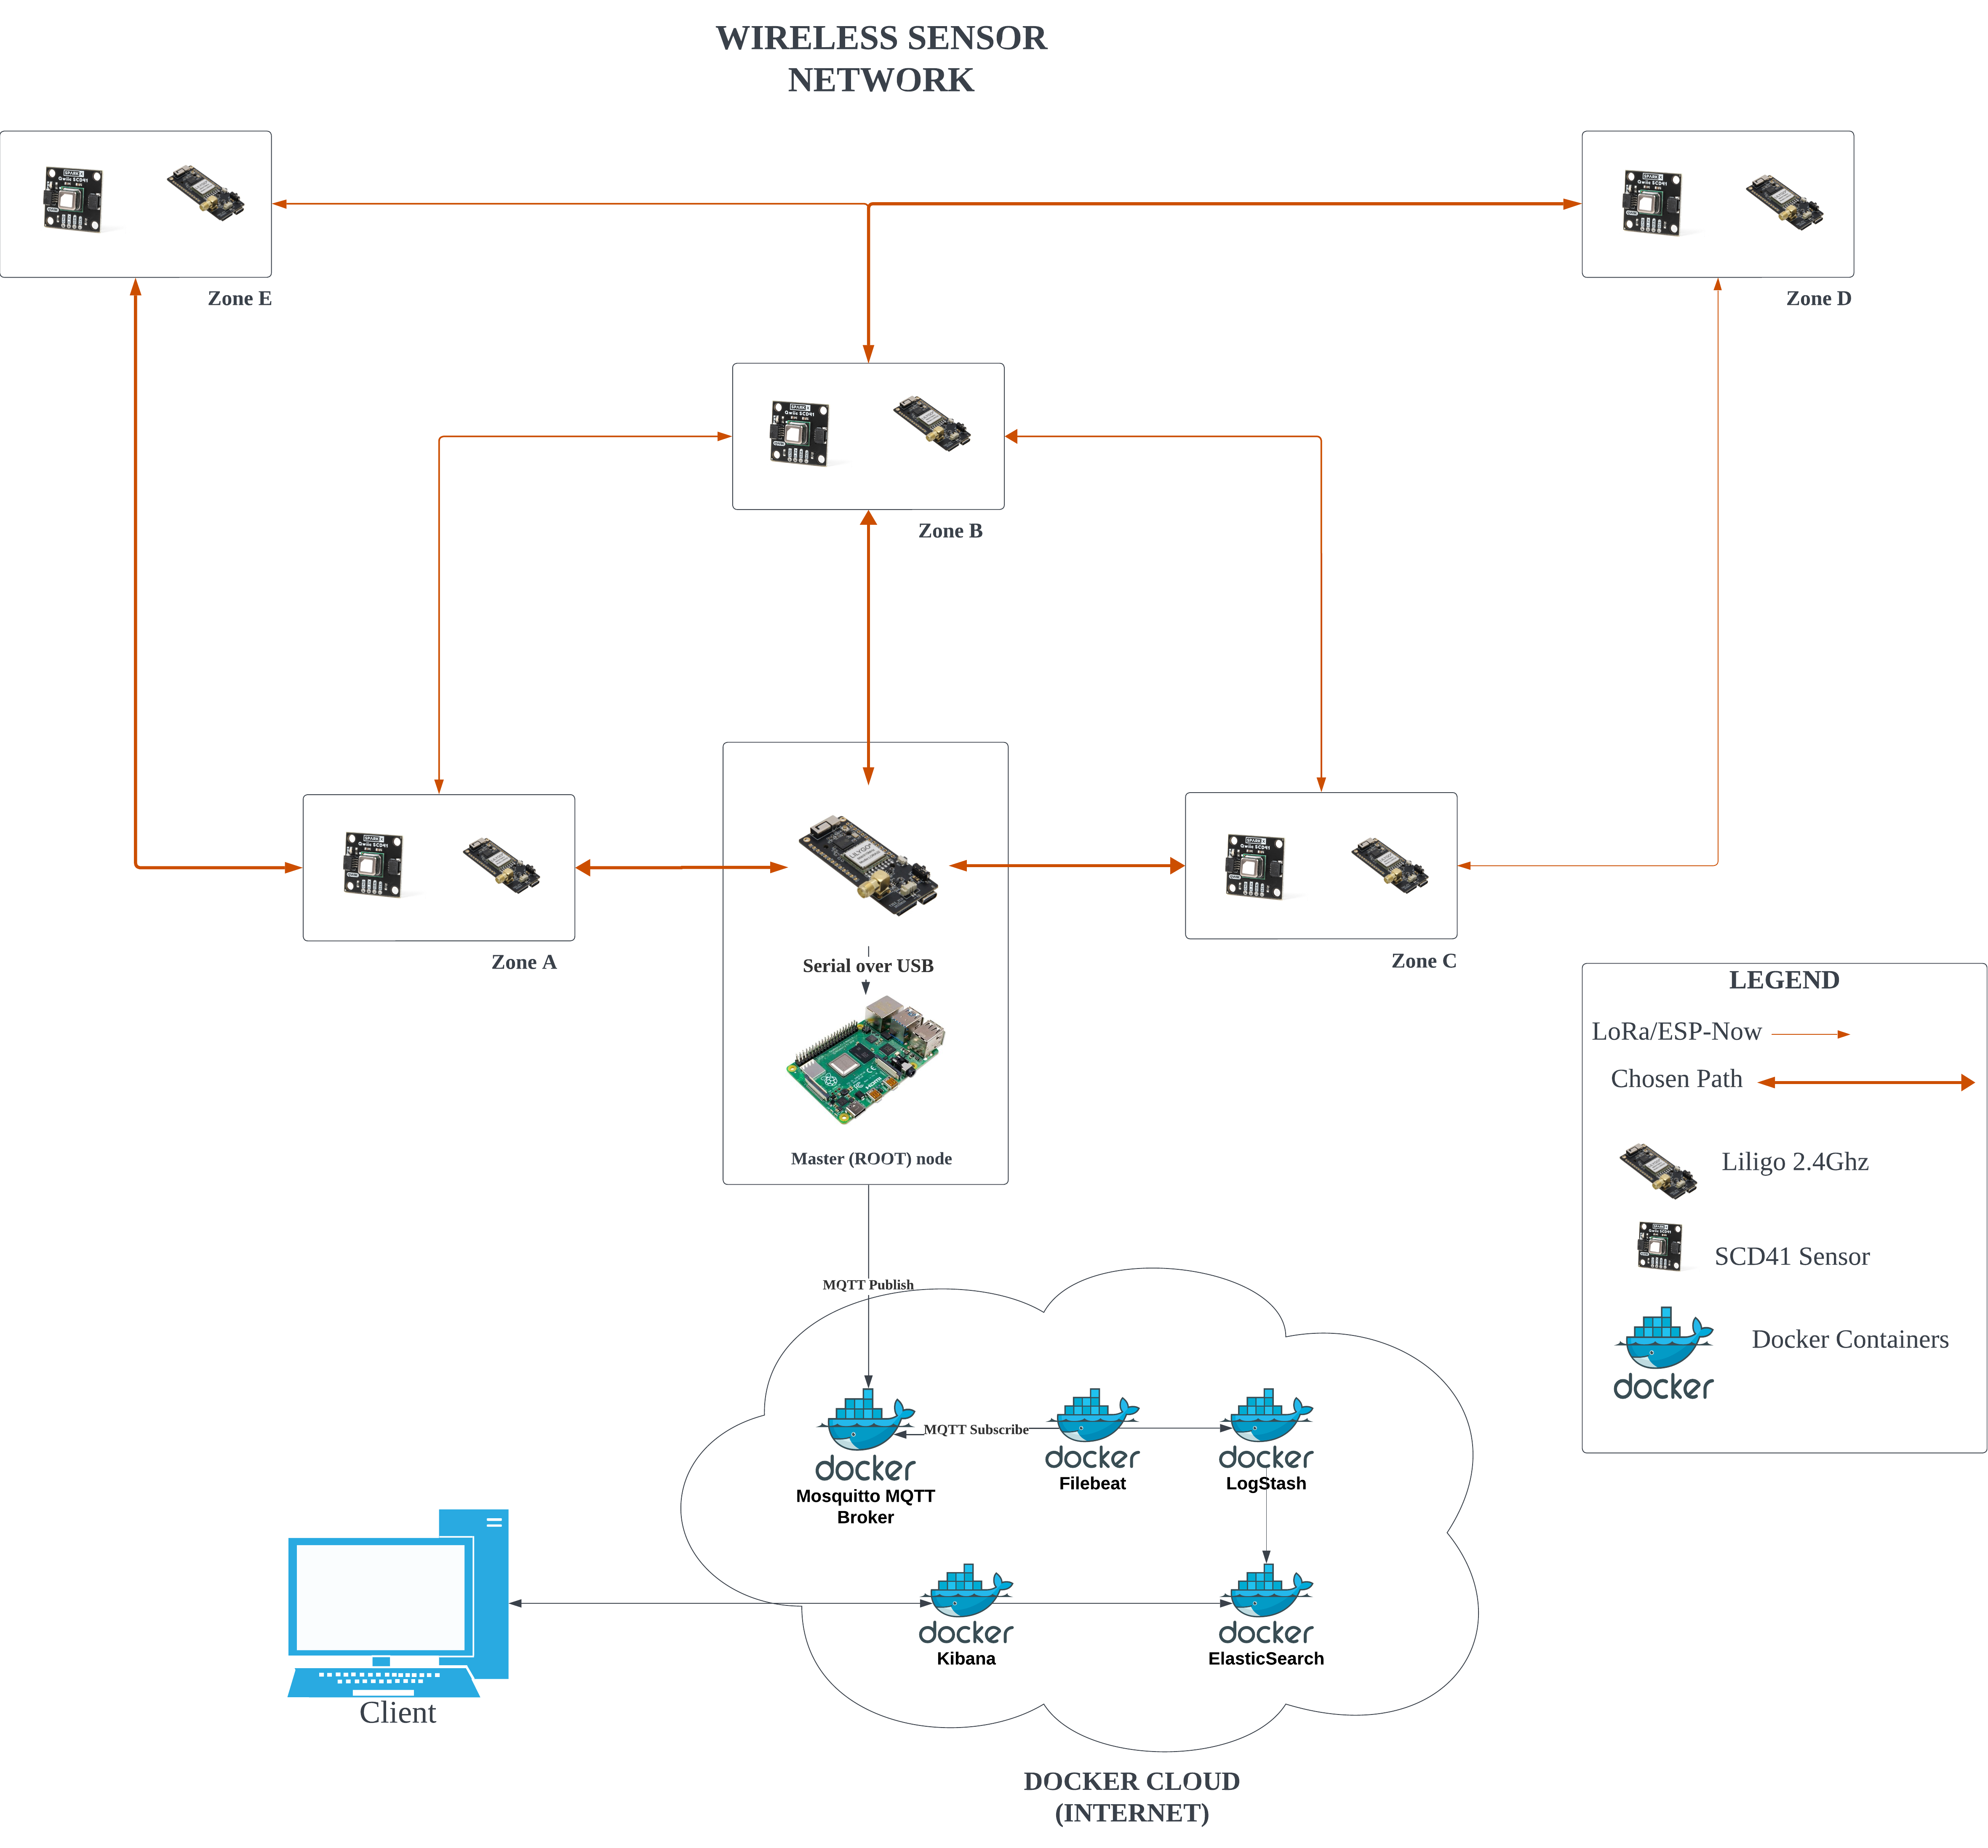
\includegraphics[width=0.35\textwidth]{./Figures/architecture.png}
  \end{center}
  \caption{Proposed System Architecture}\label{architecture}
\end{figure}

% Shorten if required
This system architecture is meticulously crafted to efficiently collect and analyze data within a Wireless Sensor Network (WSN) mesh. The architecture encompasses two principal components: the WSN mesh and the Data Collection Sink.

The WSN mesh constitutes sensor nodes equipped with Liligo T3S3 LoRa 2.4Ghz modules, facilitating inter-node communication via ESP-Now and LoRa protocols. This setup ensures optimal node discovery and routing, essential for seamless data transmission within the mesh.

The Data Collection Sink, a pivotal aspect of the architecture, comprises several interconnected components. At its core lies the Root Node, functioning as the master node within the WSN mesh. This Root Node establishes a vital link with the MQTT broker using a Raspberry Pi 4b, serving as the conduit for data transmission from the mesh to the subsequent processing stages.

Facilitating communication between the Root Node and data processing components is the MQTT Broker, realized through the Mosquitto software encapsulated within a Docker container. This broker plays a pivotal role in ensuring seamless data flow between the WSN mesh and downstream processing units.

The backbone of data processing and analysis within this architecture is the ELK Stack, comprising Filebeat, Logstash, and Elasticsearch. Filebeat, contained within a Docker environment, serves to gather data from the MQTT broker. Subsequently, Logstash, also deployed as a Docker container, undertakes the parsing and transformation of collected data before forwarding it to Elasticsearch. The latter, functioning as a robust search and analytics engine within its Docker container, serves as the repository for processed data.

The data flow within this architecture is orchestrated as follows: sensor nodes within the WSN mesh capture environmental data, which is then routed through ESP-Now and LoRa protocols towards the Root Node. From here, the data is relayed to the MQTT broker via a Raspberry Pi 4b. Filebeat, operating within a Docker container, subscribes to the MQTT broker to receive incoming data, which is subsequently processed and transformed by Logstash before being stored in Elasticsearch for visualization and analysis through Kibana.

Key points of this architecture include the utilization of ESP-Now and LoRa protocols for efficient WSN mesh communication, the pivotal role of the MQTT broker in facilitating communication between the WSN mesh and data processing components, the comprehensive data processing and analysis capabilities offered by the ELK Stack, and the efficient isolation and management of software components through Docker containers.

This architecture presents a streamlined and efficient approach for collecting and analyzing data within a WSN mesh, rendering it suitable for a myriad of applications requiring real-time data insights.


\subsection{Prototyping}\label{prototyping}
For prototyping, our strategy involves deploying sensor nodes equipped with the Liligo T3S3 Lora 2.4Ghz module. These nodes will utilize ESP-Now and LoRa Protocols for seamless communication. One node will be connected to the SCD41 Sensor, while others will generate synthetic data. The root node will establish a connection to the sink via MQTT, ensuring smooth data collection, analysis, and visualization. As an enhancement, we aim to implement protocol switching to adapt to fluctuating network conditions.

We intend to develop a modified algorithm (\textbf{DSR}) for each protocol. Each protocol mesh will include a common master node, configured with Message Queueing Technology (MQTT). This master node will interface with the backbone ELK Stack through Mosquitto MQTT Broker and filebeat with Elasticsearch for data aggregation. Kibana will be used for visualization.

\subsubsection{ESP-Now Prototype}

In crafting a sophisticated network for environmental monitoring, our collective effort harnessed the combined strengths of the ESP-NOW protocol and the Dynamic Source Routing (DSR) algorithm. This integrated approach was strategically chosen to navigate the intricate challenges associated with collecting and analyzing environmental data in real time. Engineered to deliver exceptional efficiency, flexibility, and scalability, the network stands poised to fulfill the stringent demands of a wide array of environmental monitoring projects.

The initial phase involved setting up ESP32 modules to operate with ESP-NOW, a protocol distinguished by its minimal power usage and effective direct communication features. This choice was motivated by the need for a system capable of operating in energy-constrained environments while maintaining reliable data transmission over short distances. The integration of environmental sensors, such as those for measuring temperature, humidity, and air quality, was a critical step in enabling the network to collect a wide range of data, vital for comprehensive environmental analysis.

To enhance the network's adaptability and efficiency in data routing, we will develop a custom implementation of the Dynamic Source Routing (DSR) algorithm across the devices. DSR's flexible, on-demand routing mechanism will allow the network to dynamically adjust to changes and maintain data flow when required, even in the face of node failures or alterations in network topology. This will ensure uninterrupted collection and transmission of environmental data, a key requirement for real-time monitoring applications.

In our planned setup using ESP-NOW, each peer node will regularly collect data from its SCD41 sensor. It will then consult its peer list, which will serve as a routing table, containing only the MAC addresses of the root node and those peer nodes that are either directly linked to the root node or have knowledge of the route to it. The node will then send the data from the SCD41 sensor to an appropriate node available in its peer list.

Should the peer list be empty, indicating there are no known routes, the node will initiate a route discovery process by sending out a broadcast request to surrounding nodes. When a node receives such a request, it will respond if it knows the way to the root node. The node that made the request will update its peer list with this new route information from any responder. This route discovery will continue until all neighbouring nodes have been discovered. We will also implement a hop count list to refine routing efficiency, allowing the peer node to choose the route with the shortest path to the root node to ensure the most efficient data transmission within our routing framework.

Another pivotal component of our system will be the central ESP32 module, designated as the master node. This module will serve a dual purpose: it will act as a receiver for data collected via ESP-NOW from the sensor-equipped nodes and as a transmitter, forwarding this data to a cloud service or server via WiFi using the MQTT protocol. This dual functionality will enable seamless integration of the sensor network with internet-based data processing and analysis tools, extending the capabilities of our monitoring system beyond local data collection.


\subsubsection{LoRa Prototype}

In our planned deployment of a LoRa mesh network, distinct from our ESP-NOW prototype, we aim to construct a network architecture that features a central node equipped with internet capabilities and several leaf nodes to establish the mesh. Every node within this architecture will be assigned a distinct identifier, possibly through methods like MAC Address, to assure uniqueness throughout the network. The central node will facilitate network coordination and data transmission using the MQTT protocol, while the leaf nodes will focus on tasks such as sensing and data gathering.

Upon starting up the master nodes and leaf nodes for setup, the master node will start listening for a "Discovery message" (DM). This DM will be structured to contain a message type. The leaf nodes broacast its DM to its neighbouring nodes. When a node receives a DM, if its route table is not empty, it sends a reply with its MAC address and level. When a leaf node that sends out a DM receives a "Discovery Reply Message" (DRM), it save only the route with the lowest level.

After saving the the address and level of the peer node RDM a leaf node has received, the node raises its node level by one, indicating that it is one hop further from the master node or from a known route to the master node. The node then broadcast its DM to its surrounding nodes. Nodes will ignore messages with a level higher than itself. This process will continue until the timer ends and all niehgbouring peer routes have been stored in each node's "routing table" (RT), lining up multiple potential routes.

For data transmission, the leaf node will pick the first route saved in its routing table and now send the message packet to that neighbouring peer. The message sent will be successful if it receives a "data reply message" (DRM) and the message passing continue down each level until the master node. The node will try resending the message packet via a different route in its RT, making use of various DM to find another viable path.

In our LoRa32 DSR mesh network, the master node acts as the central hub, collecting data from leaf nodes distributed throughout the network. It then efficiently transmits this data to our server for visualization and analysis. This pivotal role enables real-time monitoring and informed decision-making based on the insights gained from the data collected by our LoRa mesh network.

To optimise our LoRa mesh to better suit our project needs, we propose several strategies aimed at enhancing energy efficiency, reliability, and fault tolerance. By developing tailored routing algorithms and leveraging multi-path routing techniques, we aim to achieve these objectives while maintaining the scalability and adaptability inherent in LoRa networks.

Energy-Effecient routing can be achieved by saving and prioritising the use of shorter hops to the master node only swapping to other routes in the case of neighbouring node failure. By selecting paths with smaller hop counts, we can reduce transmission power and decrease energy consumption during data forwarding.

Multi-path routing ensures reliability and fault tolerance in our LoRa mesh network. to achieve this, multiple routes can be stored in the routing table aside from the shortest route hop discovered during route discovery phase.

\subsubsection{Elasticsearch and Kibana Integration}

In the proposed network architecture, each protocol node will incorporate a central master node equipped with a Liligo MCU, seamlessly connected to a Raspberry Pi 4 via USB. A dedicated script running on the Raspberry Pi will efficiently manage the serialization and transmission of serial data to the server using MQTT (Message Queueing Telemetry Transport), ensuring seamless integration with the ELK Stack infrastructure. The combination of Mosquitto MQTT Broker and Filebeat will facilitate streamlined data aggregation and storage management, while Kibana will serve as the intuitive visualization interface.

Data received from the LoRa/ESP-Now protocols will undergo serialization into JSON format before being dispatched to a designated topic on the MQTT Broker through the Raspberry Pi.

The deployment of the ELK Stack and MQTT will be orchestrated using Docker Compose, selected for its straightforward setup and deployment processes. Filebeat will operate as an MQTT Client, subscribing to a predefined topic to capture data packets transmitted from the master node. Subsequently, it will convert this data into JSON format and transmit it to Elasticsearch for storage and indexing. Kibana will then retrieve the data from the database, presenting it on the dashboard for clear visualization. Networking components will be seamlessly integrated within the Docker Compose environment.

In an optimal scenario, the master node will supervise a limited number of interconnected devices, typically ranging from 10 to 15 nodes, organized in either a tree or mesh structure. It will efficiently aggregate, organize, and transmit received data to the MQTT Broker, where Filebeat will undertake further processing. As a proof of concept, the mesh Wireless Sensor Network (WSN) will initially consist of a small number of nodes and one master, with data streams flowing from the master to the Mosquitto Broker for centralized collection.


\subsection{Testing}\label{testing}
In our upcoming system evaluation, we will start with unit testing on sensor nodes to confirm their communication and data generation capabilities by testing protocols between nodes. This will be followed by integration testing to assess the Wireless Sensor Network (WSN) Mesh's interoperability and its ELK stack integration, confirming efficient data transmission to the sink node. To further assess the system's adaptability and endurance, we will undertake stress testing under conditions of intense load. The outcomes of these tests are expected to demonstrate successful intra-mesh communication, reliable data conveyance to the sink, and overall system integrity, confirming our system's readiness for deployment.

Building on this foundation, our forthcoming evaluations will concentrate on meticulously analyzing the system's throughput and power consumption across both peak and normal operational phases. For measuring throughput, we will conduct a series of structured tests, using the number of packets received or transmitted over a set duration, to evaluate the data transmission capabilities of the WSN Mesh protocols across different scenarios, from optimal to high-traffic conditions. This entails systematically increasing the data load to gauge the system's capacity and pinpoint any potential bottlenecks.

Simultaneously, our approach to assessing power consumption involves real-time monitoring of the sensor nodes' energy usage across different operational states. Utilizing the S1 Energy Socket, we aim to capture and compare the power demands during idle, normal, and peak activity periods. This detailed power usage profiling over time is designed to shed light on the system's energy efficiency and spotlight areas for potential optimization.

This integrated testing framework, leveraging both simulation tools and real-world environments, is devised to offer a holistic evaluation of the system's performance and operational efficiency. By rigorously verifying that the system meets our defined benchmarks for throughput capacity and energy consumption, we ensure its suitability for widespread deployment across varied contexts, underscoring our commitment to delivering a robust and efficient solution.
